\section[تمرین چهارم: تشخیص چهره \lr{(Olivetti Faces)}]{\faUserCheck\ \ تمرین چهارم: تشخیص چهره \lr{(Olivetti Faces)}}

\begin{stepbox}

\field{خلاصه پیاده‌سازی و مصورسازی مجموعه داده}{
در این تمرین، مجموعه داده چهره‌های \lr{Olivetti} شامل ۴۰ فرد متمایز (مجموعاً ۴۰۰ تصویر گریس‌کیل $64 \times 64$) با نسبت ۸۰-۲۰ به داده‌های آموزش و آزمون تقسیم شد. جهت بررسی ساختاری و تنوع چهره‌ها، تصویر اولین نمونه از هر ۴۰ شخص استخراج و در یک ساختار منظم مصورسازی شد:

\vspace{0.4cm}
\begin{center}
    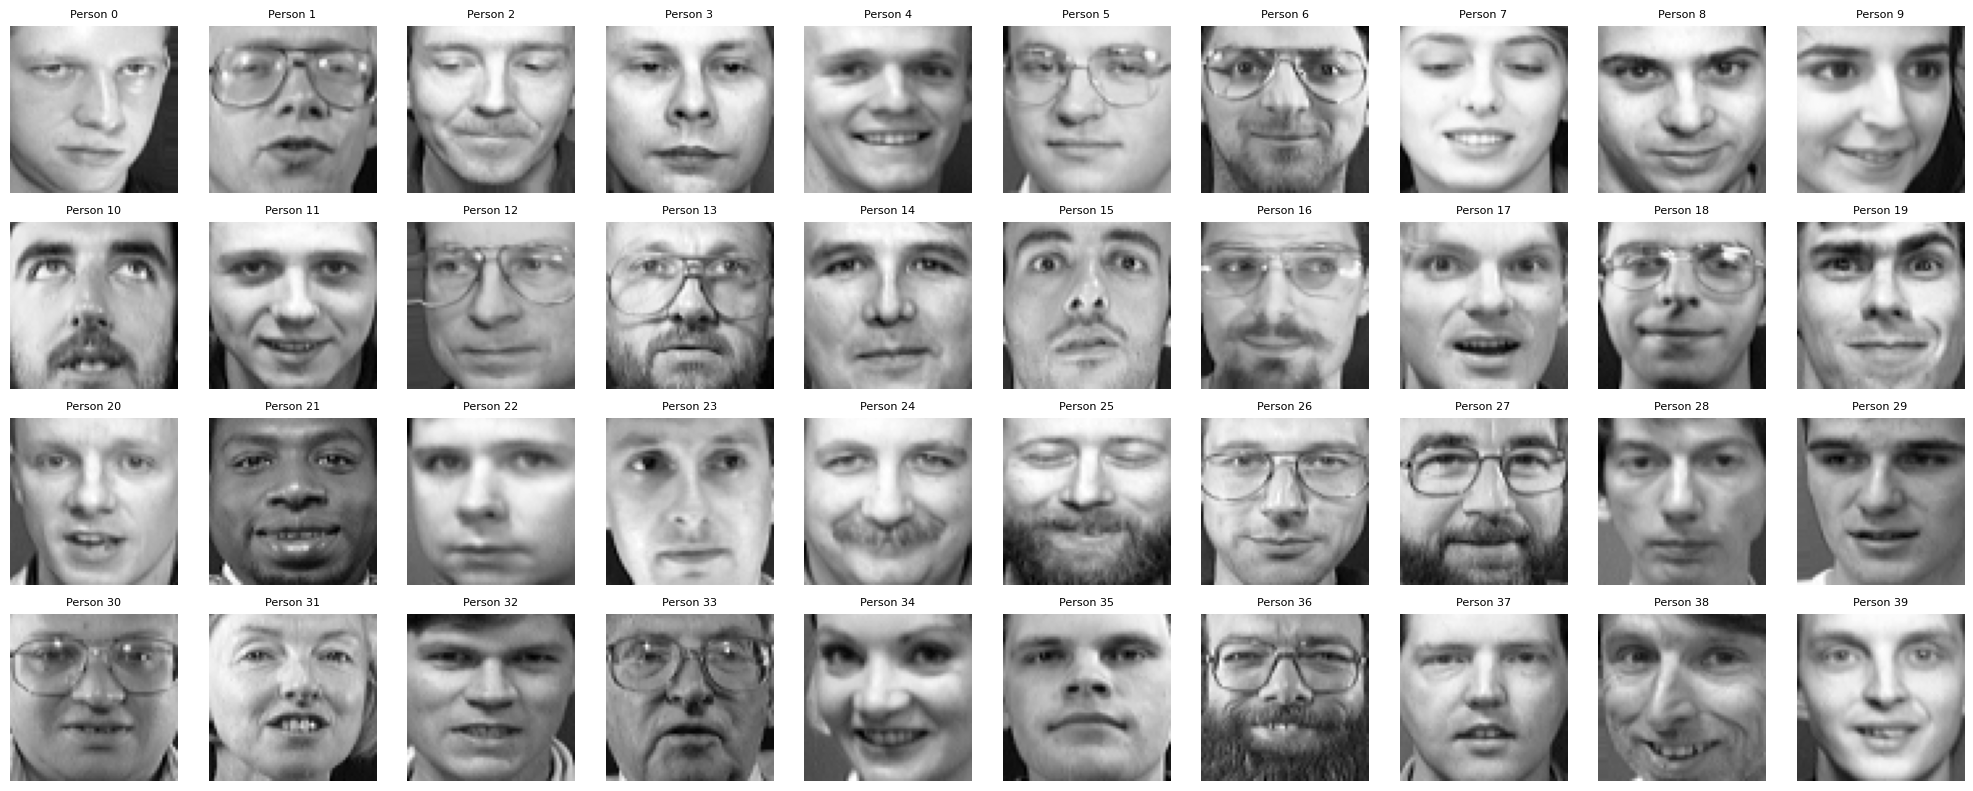
\includegraphics[width=0.85\textwidth]{images/olivetti_faces_grid.png} % نام فایل گرید چهره‌ها را مطابق خروجی پایتون خود تنظیم کنید
    \captionsetup{hypcap=false}
    \captionof{figure}{گرید تصاویر چهره‌های ۴۰ فرد متمایز در مجموعه داده Olivetti Faces}
    \label{fig:olivetti_faces}
\end{center}
}

\field{ارزیابی و مقایسه مدل‌های کلاسیک}{
عملکرد سه مدل یادگیری ماشین روی فضای ویژگی اصلی (ابعاد خام ۴۰۹۶ پیکسلی) مورد ارزیابی قرار گرفت. نتایج دقت به دست آمده روی داده‌های تست به شرح زیر است:
\begin{itemize}
    \item \textbf{ماشین بردار پشتیبان (\lr{SVM}) با کرنل \lr{RBF}:} به \textbf{دقت فوق‌العاده $96.25\%$} دست یافت. این مدل به دلیل توانایی بالا در نگاشت داده‌های با ابعاد بالا به فضایی با تفکیک‌پذیری بهتر، بهترین عملکرد را نشان داد.
    \item \textbf{جنگل تصادفی (\lr{Random Forest}):} به \textbf{دقت پایدار $95.0\%$} رسید که نشان‌دهنده قدرت بالای انسمبل‌های بگینگ در مدیریت نویزهای پیکسلی است.
    \item \textbf{الگوریتم \lr{AdaBoost}:} به \textbf{دقت بسیار ضعیف $16.25\%$} سقوط کرد که نشان‌دهنده پدیده کم‌برازش (\lr{Underfitting}) شدید است.
\end{itemize}
}

\field{ریشه‌یابی ضعف AdaBoost و بهبود آن با PCA و درخت‌های عمیق‌تر}{
دلیل افت شدید عملکرد \lr{AdaBoost} خام دو مسئله بود: اول ابعاد بسیار بالای داده‌ها (۴۰۹۶ پیکسل) که مدل بوستینگ را گیج می‌کند، و دوم استفاده پیش‌فرض از درخت‌های با عمق ۱ (\lr{Decision Stumps}) که برای تفکیک ۴۰ کلاس پیچیده چهره کاملاً ناتوان هستند. برای حل این مشکل، دو گام اساسی در کد پیاده‌سازی شد:
\begin{enumerate}
    \item \textbf{کاهش ابعاد با \lr{PCA}:} ابعاد ویژگی‌ها از ۴۰۹۶ به ۱۵۰ مولفه اصلی بهینه‌شده کاهش داده شد تا نویز برطرف شده و فضا فشرده شود.
    \item \textbf{افزایش عمق مدل‌های پایه:} درخت تصمیم پایه‌ی \lr{AdaBoost} از عمق ۱ به \textbf{عمق ۳} ارتقا یافت تا توانایی یادگیری مرزهای غیرخطی را پیدا کند.
\end{enumerate}
\[ \text{\textbf{نتیجه بهبود:}} \quad \text{جهش چشمگیر دقت مدل \lr{AdaBoost} از } 16.25\% \text{ به } \mathbf{57.5\%} \]
}

\field{راهکارهای پیشنهادی برای ارتقای بیشتر نتایج}{
برای رساندن دقت مدل‌ها به مرز ۱۰۰٪، راهکارهای زیر به عنوان فازهای توسعه آتی پیشنهاد می‌گردند:
\begin{itemize}
    \item \textbf{تنظیم ابرپارامترها (\lr{Hyperparameter Tuning}):} اعمال فرآیند \lr{GridSearchCV} بر روی عمق درخت‌های انسمبل، تعداد تخمین‌زننده‌ها و نرخ یادگیری (\lr{Learning Rate}) در الگوریتم بوستینگ.
    \item \textbf{افزایش داده‌ها (\lr{Data Augmentation}):} با توجه به اینکه از هر فرد تنها ۱۰ تصویر در دسترس است، مدل‌ها مستعد بیش‌برازش هستند. اعمال تغییرات جزئی نظیر چرخش‌های کم، زوم و تغییرات روشنایی روی تصاویر آموزشی می‌تواند پایداری مدل را تضمین کند.
    \item \textbf{بهره‌گیری از یادگیری عمیق (\lr{CNN}):} استفاده از شبکه‌های عصبی پیچشی به دلیل توانایی ذاتی در استخراج ویژگی‌های سلسله‌مراتبی و حفظ همبستگی فضایی پیکسل‌ها، گزینه‌ای بی‌نقص برای این سطح از تشخیص چهره است.
\end{itemize}
}

\end{stepbox}